\documentclass[smallextended]{svjour3}

\input{setup}

\definecolor{dkgreen}{rgb}{0,0.6,0}
\definecolor{gray}{rgb}{0.5,0.5,0.5}
\definecolor{mauve}{rgb}{0.58,0,0.82}
\lstset{frame=tb,
	language=Java,
	aboveskip=3mm,
	belowskip=3mm,
	showstringspaces=false,
	columns=flexible,
	basicstyle={\small\ttfamily},
	numbers=none,
	%numberstyle=\tiny\color{gray},
	%keywordstyle=\color{blue},
	%commentstyle=\color{dkgreen},
	%stringstyle=\color{mauve},
	breaklines=true,
	breakatwhitespace=true,
	tabsize=3
}


\newcommand{\specialcell}[2][c]{%
	\begin{tabular}[#1]{@{}c@{}}#2\end{tabular}}

\usepackage{multirow}
\usepackage{graphicx}
\usepackage{amsmath,amssymb,amsfonts}
\usepackage{algorithmic}
% \usepackage{caption}
\usepackage{subcaption}
\usepackage{subfig}
\usepackage{textcomp}
\usepackage{xcolor}
\usepackage{tcolorbox}
\usepackage{booktabs}
\usepackage{listings}
\usepackage{color}  
\usepackage{textcase}
\usepackage{setspace}
\usepackage[flushleft]{threeparttable}
\usepackage{flushend}
\usepackage{float}
\usepackage{courier}
\usepackage{multirow}
% \usepackage{hyperref}
\usepackage{makecell}


\usepackage[round,sort]{natbib}

\usepackage{array}
\newcolumntype{L}[1]{>{\raggedright\let\newline\\\arraybackslash\hspace{0pt}}m{#1}}
\newcolumntype{C}[1]{>{\centering\let\newline\\\arraybackslash\hspace{0pt}}m{#1}}
\newcolumntype{R}[1]{>{\raggedleft\let\newline\\\arraybackslash\hspace{0pt}}m{#1}}

\newcommand{\shuang}[1]{\textcolor{black}{{#1}}}
\newcommand{\red}[1]{\textcolor{red}{#1}}


\begin{document}

\title{Beyond Merge Rate: Measuring Performance of Autonomous Coding Agents}

\author{Ziyi Yin \and
	      Jinfu Chen\textsuperscript{$\ast$} \thanks{\textsuperscript{$\ast$}Corresponding author} \and
        Derui Zhu \and  
	    Jifeng Xuan  
}

\institute{Ziyi Yin, Jinfu Chen, Jifeng Xuan\at
	School of Computer Science\\
	Wuhan University\\
	Wuhan, China\\
	\email{\{ziyiyin, jxuan\}@whu.edu.cn} \\\\
    Jinfu Chen\at
	School of Computer Science \& Key Laboratory of Intelligent Sensing System and Security (Ministry of Education)\\
	Wuhan University \& Hubei University\\
	Wuhan, China\\
	\email{jinfuchen@whu.edu.cn} \\\\ 
	Derui Zhu\at
	Department of Software Engineering\\
	Rochester Institute of Technology\\
	Rochester, NY, US\\
	\email{dxzvse@rit.edu} 
}

\date{Received: date / Accepted: date}

% make the title area
\maketitle
\begin{abstract}
The integration of Large Language Models (LLMs) into software development ...

\end{abstract}

\keywords{Agentic Software\and Software Performance\and Performance Engineering \and Large Language Models}

\section{Introduction} \label{sec:intro}
\label{intro}
The integration of LLMs into software development tools has introduced a new era of AI-powered coding assistants. These LLM-based tools, such as GitHub Copilot, Copilot Chat, ChatGPT, and CodeWhisperer ....
While tools like Copilot, and DeepSeek-Coder offer the potential to enhance developer productivity, ensuring the quality of the generated code remains a crucial area of investigation. Prior research has extensively studied and reported challenges related to correctness~\citep{DBLP:conf/msr/NguyenN22,wang2025understandingcharacteristicscodegeneration}, security and privacy associated with code generated by LLMs. 

 Autonomous coding agents now submit agentic PRs at scale and are demonstrably weaker than humans on acceptance, especially on performance tasks. 
 
 Prior work on agentic performance PRs reports a rejection-rate penalty (36.5\% vs. 22.7\%) and builds a topic taxonomy. However, ...
 
 We study 1,219 agent-authored performance PRs and decompose both ends of the outcome distribution. Present the results of our study...
 
To facilitate research reproducibility, we make the original datasets, scripts available in our replication package\footnote{link}. 
Our contributions are summarized below.
\begin{itemize}
   
    \item \textbf{Performance assessment of agent-generated PR:} We systematically evaluated the .... 
    \item \textbf{Root causes of AI-generated code:} We qualitatively analyzed the root causes of performance ...
    \item \textbf{XXXX:} We explored ...
\end{itemize}

The rest of this paper is organized as follows. Section~\ref{background} introduces XXX. Section~\ref{approach} presents our case study setup. Section~\ref{result} presents detailed results of our research questions and findings. Section~\ref{discussion} discusses the implications of our findings. Section~\ref{threats} discusses the threats to the validity of our study. Section~\ref{related} presents related prior studies. Section~\ref{conclusion} summarizes the conclusion of our study.

\section{Background and example}
\label{background}
In this section, we first introduce five LLM-based agents, GitHub Copilot, ... We then present a motivating example of ....

\subsection{Agentic Software Engineering}
Introduce AI-Assisted Software Engineering and Agentic Software Engineering


\subsection{Autonomous Coding Agent in Software Engineering}


\subsection{An example of performance challenges in AI-generated code}

\begin{figure}
\centering
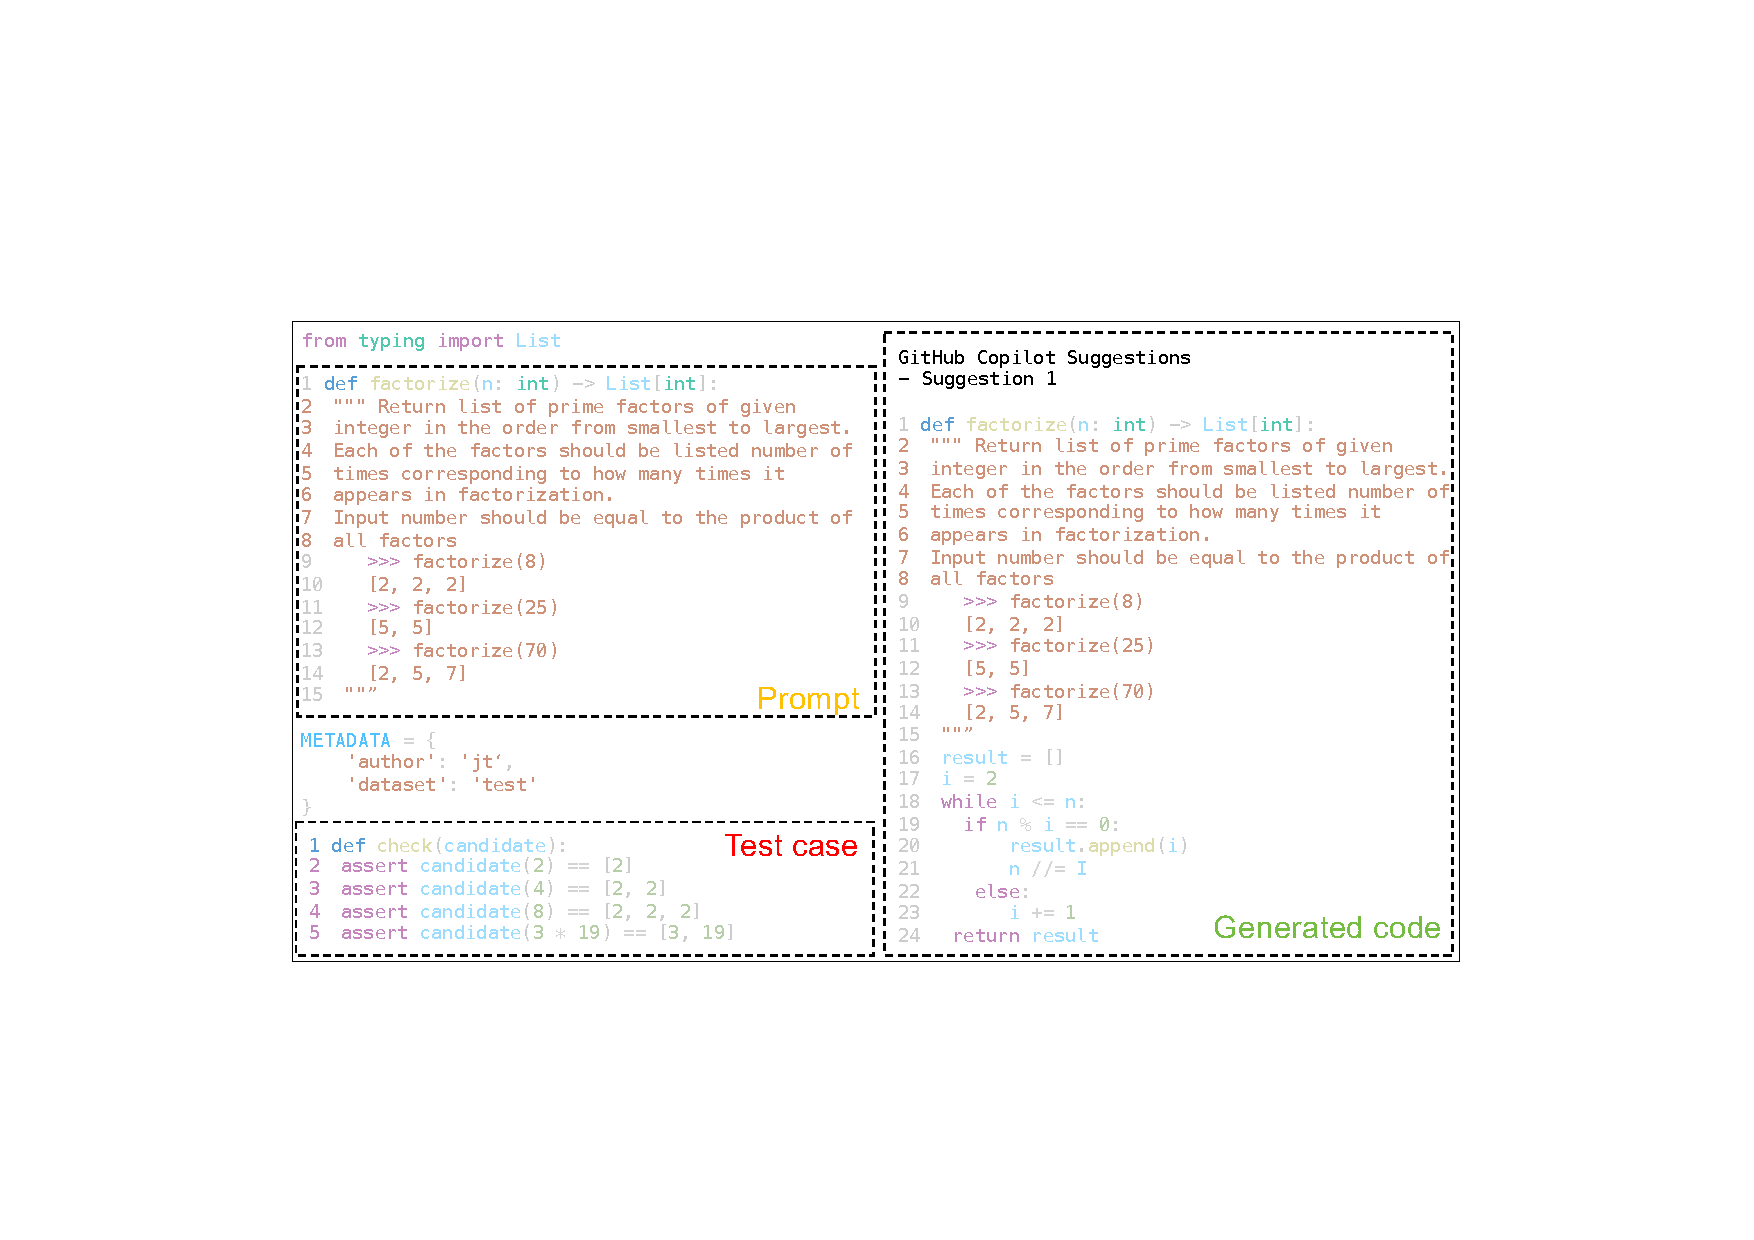
\includegraphics[width=0.95\columnwidth]{pics/background/update_example.pdf}
% \vspace{-0.1cm}
\caption{An example of generating the function by Copilot.}
% \vspace{-0.1cm}
\label{copilot-example}
\end{figure}


\section{Study setup}
\label{approach}
In this section, we present our case study setup. In particular, we present the datasets used in our case study and our experimental setup to collect ...

\subsection{Corpus construction}
AIDev dataset - LLM-based performance detection - 1,219 performance PRs across 447 repositories and five agents

The overview of datasets is shown in Table~\ref{dataset}.

\begin{table}
\centering
\caption{\shuang{Overview of datasets used in our study}}
\label{dataset}
\resizebox{0.9\columnwidth}{!}{  
\begin{tabular}{ccccc}
\toprule
Dataset   & Language & \#Instances & Year & Reference \\ \toprule
HumanEval & Python   & 164        & 2021 &      \cite{chen2021evaluating}    \\ 
AixBench  & Java     & 187        & 2022 &   \cite{hao2022aixbench}        \\ 
MBPP      & Python   & 974        & 2021  &   \cite{austin2021mbpp}       \\
EvalPerf  & Python   & 118        & 2024  &   \cite{DBLP:journals/corr/abs-2408-06450}       \\\bottomrule
\end{tabular}
}
\end{table}



\subsection{Experimental setup}
In this subsection, we describe the process of collecting the generated PRs and performance data for each question in our study datasets. Figure~\ref{overview} illustrates the overall process of our approach. We follow four steps to collect the needed data. In the first step, we .... 

\begin{figure*}[tbh]
\centerline{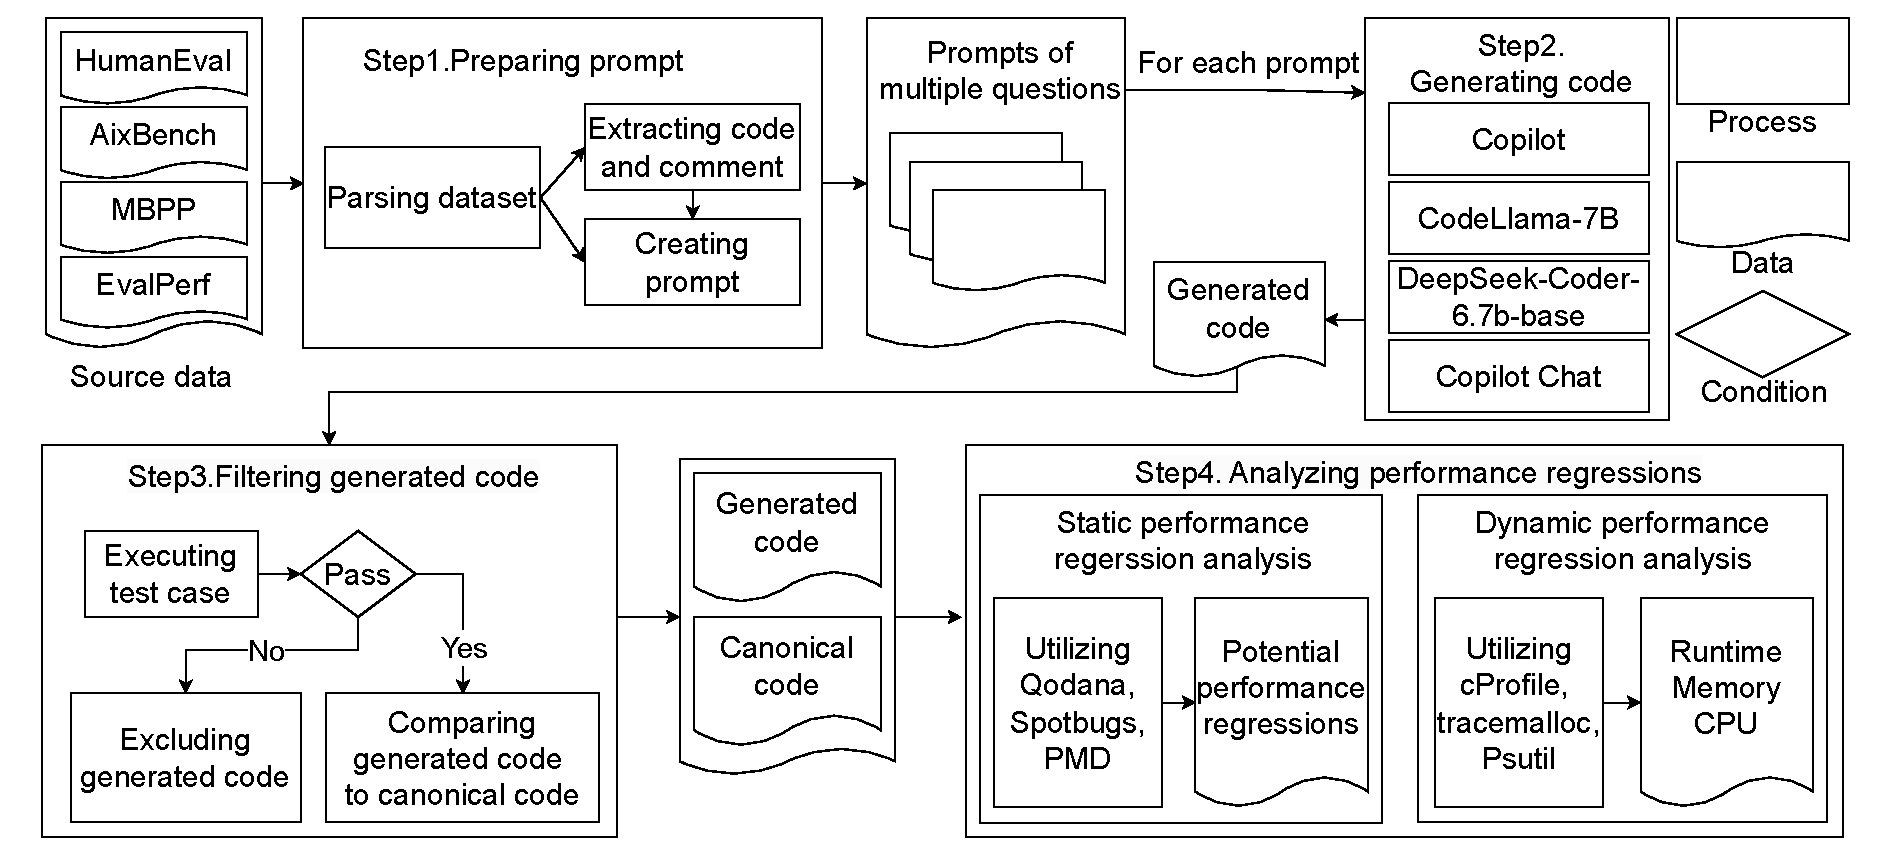
\includegraphics[width=1\textwidth]{./pics/approach/overview-new-new.drawio.pdf}}
\caption{\shuang{An overview of our approach to collecting data.}}
\label{overview}
\end{figure*}

{\textbf{Step 1: XXX.}} 


{\textbf{Step 2: Generating code.}}
In this step, we use

\textbf{Step 3. Filtering performance-related PRs.}
In this step, we filter 


\textbf{Step 4. Analyzing PR data.}
\label{analyze}

The hardware configuration for the experiment includes an Intel Core i9-13900K processor, 128 GB of RAM, 1 TB SSD for primary storage, and 8 TB HDD for secondary storage, and the system operates on Ubuntu 22.04.4 LTS. By following the experimental setup, we aim to achieve a thorough and systematic evaluation of the performance regressions of AI-generated code, considering both static and dynamic aspects, and providing actionable insights for code optimization and tool improvement.

% \section{Case Study Setup} \label{sec:casestudysetup}
To study the effectiveness of our approaches for detecting performance regressions under varying workloads, we perform case studies on two open-source systems\footnote{Our experimental setup, workloads, and results are shared online \url{https://github.com/senseconcordia/EMSE2020Data} as a replication package.}. In this section, we first present the subject systems. Then, we present the workloads applied to the systems, the experimental environment, and performance issues. Finally, we present the choices of machine learning models that are used in our approaches. 

\subsection{Subject systems}
We evaluate our approaches on two open-source systems, namely OpenMRS and Apache James. We also discuss the successful application of our approach in System X, a large-scale industrial system that provides government-regulation related reporting services (in Section~\ref{sec:deploymentinindustry}). Apache James is a Java-based mail server. OpenMRS is an open-source health care system that supports customized medical records and it is wildly used in developing countries. The two open-source subject systems and the industrial system are all studied in prior research~\citep{Yao:2018:LSL:3184407.3184416, DBLP:conf/icst/GaoJBL16} and cover different domains, which ensures that our findings are not limited to a specific domain. The details of the two open-source subject systems and the industrial system are shown in Table~\ref{tab:subjects}. 

Both two open-source subject systems and the industrial system are CPU-intensive. Besides, CPU is usually the main contributor to server costs~\citep{Greenberg:2008:CCR:1496091.1496103}. Performance regression in terms of CPU would result in the need for more CPU resources to provide the same quality of service, thereby significantly increasing the cost of system operations. 
%For example, for our industrial system (System X), CPU usage is the main concern in performance regression detection.
Therefore, in this study, we use CPU as the performance metric for detecting performance regressions. 
%\heng{Moved the CPU usage information to the end of 4.2 Subject workload design, as 1) we have not talked about the different versions here, 2) we just claimed that these systems are cpu-intensive. }
%(summarized in Table~\ref{tab:cpu_utilization}). \ian{added} We would like to note that when we observe a higher CPU usage, it may not correspond to a performance regression, while it may be just because the system has a higher workload. The influence from the workload to the CPU usage is one of the reason that we leverage performance modeling to detect performance regressions in the field.



\begin{table}[tbh]
  \centering
  \caption{Overview of the open-source subject systems and the industrial system.}
    \begin{threeparttable}
    \begin{tabular}{c|c|c|r}
    \hline
    Subjects & Versions & Domains & SLOC (K) \\
    \hline
    OpenMRS & 2.1.4 & Medical & 67 \\
    
    Apache James & 2.3.2, 3.0M1, 3.0M2 & Mail Server & 37 \\
    
    System X\tnote{*} & 10 releases in 2019 & Commercial & \textgreater 2,000 \\
    \hline
    \end{tabular}%
    \begin{tablenotes}
    \item[*] We share our experience of applying our approaches on System X in Section~\ref{sec:deploymentinindustry}.
    \end{tablenotes}
    \end{threeparttable}
  \label{tab:subjects}%
\end{table}%


% Table generated by Excel2LaTeX from sheet '___3'
\begin{table*}[htbp]
  \centering
  \tiny
  \caption{Summary of the test actions with increased appearances (the ones with $\bullet$) in different load drivers.}
    \begin{tabular}{|m{16em}<{\centering}|m{4em}<{\centering}|m{4em}<{\centering}|m{4em}<{\centering}|m{4em}<{\centering}|m{4em}<{\centering}|}
    \hline
    \multicolumn{6}{|c|}{OpenMRS} \\
    \hline
    \multicolumn{1}{|c|}{Test actions} & Load driver 1 & Load driver 2 & Load driver 3 & Load driver 4 & Load driver 5 \\
    \hline
    Creation of patients & $\bullet$   &       & $\bullet$   &       & $\bullet$ \\
    \hline
    Deletion of patients & $\bullet$   &       & $\bullet$   &       & $\bullet$ \\
    \hline
    Searching for patients & $\bullet$   & $\bullet$   &       &       &  \\
    \hline
    Editing patients &       &       &       & $\bullet$   & $\bullet$ \\
    \hline
    Searching for concepts &       &       & $\bullet$   & $\bullet$   & $\bullet$ \\
    \hline
    Searching for encounters &       & $\bullet$   & $\bullet$   &       &  \\
    \hline
    Searching for observations &       &       & $\bullet$   & $\bullet$   & $\bullet$ \\
    \hline
    Searching for types of encounters &       & $\bullet$   &       & $\bullet$   & $\bullet$ \\
    \hline
    \multicolumn{6}{c}{} \\
    \hline
    \multicolumn{6}{|c|}{Apache James} \\
    \hline
    \multicolumn{1}{|c|}{Test actions} & Load driver 1 & Load driver 2 & Load driver 3 & Load driver 4 & Load driver 5 \\
    \hline
    Sending mails with short messages and without attachments &       &       &       & $\bullet$   &  \\
    \hline
    Sending mails with long messages and without attachments & $\bullet$   & $\bullet$   & $\bullet$   &       & $\bullet$ \\
    \hline
    Sending mails with short messages and with small attachments &       &       & $\bullet$   & $\bullet$   &  \\
    \hline
    Sending mails with short messages and with large attachments &       & $\bullet$   &       &       &  \\
    \hline
    Sending mails with long messages and with small attachments &       &       & $\bullet$   &       &  \\
    \hline
    Sending mails with long messages and with large attachments & $\bullet$   & $\bullet$   &       &       &  \\
    \hline
    Retrieving entire mails &       &       &       &       & $\bullet$ \\
    \hline
    Retrieving only the header of mails & $\bullet$   &       &       & $\bullet$   & $\bullet$ \\
    \hline
    \end{tabular}%
  \label{tab:workload_difference}%
\end{table*}%



\subsection{Subject workload design}
\subsubsection{OpenMRS}
OpenMRS provides a web-based interface and RESTFul services. We used the default OpenMRS demo database in our performance tests. The demo database contains data for over 5K patients and 476K observations. OpenMRS contains four typical scenarios: adding, deleting, searching, and editing operations. We designed different performance tests that are composed of eight various test actions, including 1) creation of patients, 2) deletion of patients, 3) searching for patients, 4) editing patients, 5) searching for concepts, 6) searching for encounters, 7) searching for observations, and 8) searching for types of encounters.
%\ian{should be i.e., not e.g., right? and we need to number the actions}e.g., searches of patients, concepts, encounters, and observations, and creation, deletion and edit of patient information.
Those performance tests are different in the ratio between the actions. 
In order to simulate a more realistic workload in the field, we added random controllers and random order controllers in JMeter to vary the workload. Moreover, we also simulated the variety of the number of users and activities in the field by setting random gaps between the repetitions of each user’s activities, randomizing the order of the user activities, and setting a different number of maximum concurrent users for different workloads at different times.

Furthermore, we designed a total of five JMeter-based performance tests, each of which consists of a mixture of random workloads. % as described above. 
In particular, to drive different workloads, for each of the load drivers, we pick several different test actions and put them in an extra JMeter loop controller that iterates a random number of times to increase their appearances in the workload. Table~\ref{tab:workload_difference} shows the detailed choice of the looped actions of each load driver. 
To make sure that the two versions of the subject systems have different workloads, for one version of the system (e.g., the old version), we run four JMeter tests together to exercise the system. For the other version (e.g., the new version) of the system, we run one additional JMeter test, i.e, a total of five JMeter tests, to ensure that the two versions have undergone different workloads.
%\lizhi{Through the analysis of results, it is found that test action \emph{deletion of patients} has the largest portion of changes ranging from $2.7\%$ to $8.3\%$}

Despite the variation in the workloads, we keep our systems not saturated and running in normal conditions. The  CPU  saturation  can  be  qualified as the average CPU load increases to a very large value (e.g., 90\%) and remains for a long period of time ~\citep{10.1117/12.705735}. When the system is saturated, the services of the systems are not provided normally and the relationship between the performance of a software system (e.g.,  CPU usage) and the runtime activities may change. Besides, real software systems are usually not running under saturated conditions.  
The details of the workload, such as the CPU usage values, are shared in our replication package. 

%\lizhi{ref. R1.1 
For the OpenMRS system, we do not have any evidence showing performance regressions of specific versions. Therefore, we manually inject several performance regressions in the system. The injected performance regressions are shown in Table~\ref{tab:workloaddeisign}. 
The original version, i.e., v0 of OpenMRS does not have any injected or known performance regressions. 
We separately injected four performance regressions (heavier DB request, additional I/O, constant delay and additional calculation) on the basis of version v0. These four versions are called v1, v2, v3, and v4, respectively. The details of the injected performance regressions of OpenMRS are explained below:
\begin{itemize}
    \item[$\bullet$] \textbf{v1: Injected heavier DB request.}  We increased the number of DB requests in the code responsible for accessing the database in OpenMRS. This performance issue will increase the CPU usage of the MySQL server.
    \item[$\bullet$] \textbf{v2: Added additional I/O access.} Since accessing I/O storage devices (e.g., hard drives) are usually slower than accessing memory, we added redundant logging statements to the source code that is frequently executed. The execution of the logging statements will introduce performance regression.
    \item[$\bullet$] \textbf{v3: Created constant delay.} We added the delay bug in the frequently executed code, which creates a blocking performance issue.
    \item[$\bullet$] \textbf{v4: Injected additional calculation.} We added additional calculations to the source code of OpenMRS that are frequently executed during the performance test.
\end{itemize}
%}

We deployed the OpenMRS on two machines, each with a configuration of Intel Core i5-2400 CPU (3.10GHz), 8 GB memory, and 512GB SATA hard drive. One machine is deployed as the application server and the other machine is deployed as the MySQL database server. We ran JMeter using the RESTFul API of OpenMRS on five extra machines with the same specification to simulate user workloads on the client side for five hours. Each machine hosts one JMeter instance with one type of workload. We used \emph{Pidstat}~\citep{pidstat} to monitor the CPU usage that is used as the performance metrics of this study.
To minimize the noise from the system warm-up and cool-down periods, we filtered out the data from the first and last half hour of running each workload. Thus, we only kept four hours of data from each performance test.

\subsubsection{Apache James}
Apache James is an open-source enterprise mail server. It contains two main actions: sending and retrieving mails. Those two actions can be further divided into many smaller actions, e.g., sending mails with or without attachments and retrieving an entire mail or only the header of the mail. In total, we built eight actions for the performance test, including 1) sending mails with short messages and without attachments, 2) sending mails with long messages and without attachments, 3) sending mails with short messages and with small attachments, 4) sending mails with short messages and with large attachments, 5) sending mails with long messages and with small attachments, 6) sending mails with long messages and with large attachments, 7) retrieving entire mails, and 8) retrieving only the header of mails.
Similar to OpenMRS, we also created a total of five different workloads, where each workload consists of a mixture of eight test actions with different ratios. 
We conduct performance tests with different versions of Apache James with varying workloads (i.e., 4 tests for one version and 5 tests for the other version). We used JMeter to create performance tests that exercise Apache James.
Different from OpenMRS, in which the performance regressions are manually injected, we performance-tested on three different versions of systems with known real-world performance issues for Apache James. Apart from the last stable version 2.3.2, there are multiple Milestone Releases for version 3.0. After checking the release notes on the Apache James website, we picked 3.0M1 and 3.0M2 to use in our study. These three selected versions have many bug fixes and performance improvements~\citep{Apache-James}. The same subjects are studied in prior research on performance testing~\citep{DBLP:conf/icst/GaoJBL16}. Table~\ref{tab:workloaddeisign} summarizes the details of performance improvements of three selected versions. 

We deployed Apache James on a server machine with an Intel Core i7-8700K CPU (3.70GHz), 16 GB of memory, and a 3TB SATA hard drive. We ran JMeter on five extra machines with a configuration of Intel Core i5-2400 CPU (3.10GHz), 8 GB memory and 320GB SATA hard drive. These JMeter instances generate multiple workloads for five hours. Similar to OpenMRS, we use \emph{Pidstat}~\citep{pidstat} to monitor the CPU usage as the performance metrics of this study. We filtered out the data from the first and last half hour of the tests to minimize the system noise.

% \subsubsection{System X}
% System X is deployed in production and is used by real users worldwide. We retrieved the execution logs and the corresponding CPU usage on a daily basis. System X is deployed in an internal production environment. Due to the NDA, we cannot reveal additional details about the hardware environment and the usage scenarios of System X.



\begin{table}[tbh]
  \centering
  \caption{Performance regressions in the studied open-source systems}
    \begin{tabular}{c|c|p{3.3cm}}
    \hline
    System & Versions & \multicolumn{1}{c}{Performance regressions} \\
    \hline
          & v0    & \multicolumn{1}{c}{Original version} \\
\cline{2-3}          & v1    & \multicolumn{1}{c}{Injected heavier DB request} \\
\cline{2-3}    OpenMRS & v2    & \multicolumn{1}{c}{Added additional I/O access} \\
\cline{2-3}          & v3    & \multicolumn{1}{c}{Created constant delay} \\
\cline{2-3}          & v4    & \multicolumn{1}{c}{Injected additional calculation} \\
    \hline
          & 2.3.2 & \multicolumn{1}{c}{Stable release version} \\
          \cline{2-3}
          Apache James & 3.0M1 & \multicolumn{1}{c}{Improved ActiveMQ spool efficiency~\citep{Apache-James}} \\
          \cline{2-3}
          & 3.0M2& \multicolumn{1}{c}{Improved large attachment handling efficiency~\citep{Apache-James}} \\
    \hline
    \end{tabular}%
  \label{tab:workloaddeisign}%
\end{table}%

\subsubsection{Generated workloads}

Our generated workloads are different across different software versions.
By conducting chi-square tests of independence between the number of different actions and the versions, we find that in both OpenMRS and Apache James, the number of different actions and the versions are not statistically independent (p-value $\ll$ 0.05), which means that the distribution of the actions are statistically different across versions. For example, for the OpenMRS system, the total number of all actions ranges from 10,673 to 22,392 across versions. In particular, the number of the \emph{deletion of patients} action has a range from 293 to 1,861 across all versions. For another example from Apache James, the number of the \emph{retrieving only the header of mails} action has a range from 411 to 25,532 across all versions. In addition, we provide the detailed numbers of each action that are sent to each version in our replication package. 




Table~\ref{tab:cpu_utilization} summarizes the average CPU utilization of each version of the systems under our generated dynamic workloads. We would like to note that when we observe a higher CPU usage, it may not correspond to a performance regression; instead, it may be just due to the system having a higher workload. The influence of the dynamic workload on the CPU usage is one of the reasons that we leverage performance modeling to detect performance regressions in the field.
The detailed CPU utilization information during the entire test time period is reported in the replication package.

% Table generated by Excel2LaTeX from sheet '___2'
\begin{table}[tbh]
  \centering
  \footnotesize
  \caption{Summary of average CPU utilization of each version in our case studies.}
 
    \begin{tabular}{c|c|c|c|c|c}
\hline    \multicolumn{6}{c}{OpenMRS} \\
\hline
    v0 (4w) & v0 (5w) & v1    & v2    & v3    & \multicolumn{1}{c}{v4} \\
    \hline
     52.03 & 52.24 & 55.55 & 53.76 & 53.05 & 55.11 \\
    \hline
    \end{tabular}%
\vspace{1em}

    \begin{tabular}{c|c|c|c}
\hline  \multicolumn{4}{c}{ Apache James} \\
\hline
     3.0M2 (4w) & 3.0M2 (5w) & 3.0M1 & 2.3.2 \\
    \hline
     0.48  & 0.51  & 3.54  & 4.89 \\
    \hline
    \end{tabular}%

  \label{tab:cpu_utilization}%
\end{table}%

\subsection{Subject models}
Our approach presented in Section~\ref{sec:approach} is not designed strictly for any particular type of machine learning models. In fact, practitioners may choose their preferred models. In this study, we study the use of six different types of models, namely linear regression, random forest, XGBoost, convolutional neural network (CNN), recurrent neural network (RNN) and long short-term memory (LSTM). In particular, for linear regression, random forest, and XGBoost, the inputs of the models are vectors whose values are the number of appearances of each log event in a time period. For CNN, RNN, and LSTM, we sort the logs in each time period by their corresponding time stamp to create a sequence as the input of the neural networks. Our XGBoost model is fine-tuned using the GridSearchCV~\citep{girdsearcv} method. Our CNN, RNN, and LSTM have three, four and four layers, respectively, and they are trained with five, five and ten epochs, respectively. The number of layers and epochs are manually fine-tuned to avoid overfitting.


% \usepackage{float}
\section{Case study results}
\label{result}
In this section, we present our case study results by answering four research questions. For each research question, we show the motivation, approach, and corresponding results of the research question.

{\color{red}Image to be added}

\subsection{RQ1: What is the outcome landscape of agent-authored performance PRs?}
\label{RQ1}

\noindent\textbf{Motivation:} 
If merge rate is the score, we first need to know what the score is averaging. Treating “closed” as “rejected by a reviewer” would invent a quality gate that many threads never contained. Treating “merged” as “reviewed and measured” would invent a performance-engineering process that most successes never entered. RQ1 maps the landscape before any path is read as skill.

\noindent\textbf{Approach:}
We report GitHub status on the full corpus (\(n=1{,}219\)). Comparative merge rates use terminal PRs (\(n=1{,}180\)). Agent rates are shown for every agent; Claude Code (\(n=38\)) is not ranked as a model comparison. Internal structure of merged and closed PRs uses the labels in the official RQ analysis. For closures we apply a mechanism partition: \emph{real rejection} (blocking review, \texttt{CHANGES\_REQUESTED}, or an explicit technical or design veto), \emph{silent abandonment} (stale, no review, author walk-away, or bot expiry), \emph{other process}, and \emph{unclear}. Open PRs enter only the corpus-level counts.

\noindent\textbf{Results:}

\textbf{The terminal merge rate is 56.8\% (670/1{,}180), but merged and closed are internally heterogeneous.} As shown in the status distribution, 670 PRs are merged (55.0\% of 1{,}219), 510 are closed (41.8\%), and 39 remain open (3.2\%). The corresponding terminal reject rate is 43.2\% (510/1{,}180).

\textbf{Agents do not share one rate.} As shown in the agent table, OpenAI Codex has a terminal merge rate of 71.7\% (451/629). Cursor has 54.5\% (48/88) and Claude Code has 61.8\% (21/34, \(n=38\) in the corpus). Copilot and Devin sit lower: 37.7\% (77/204) and 32.4\% (73/225). We report these gaps as descriptive facts. They may mix model behavior with repository choice, default patch size, and whether the agent opens unsolicited optimizations. They are not a leaderboard.

\textbf{The work sits in ordinary product layers.} The most common optimization layers are application service (201/1{,}219 = 16.5\%), build (165 = 13.5\%), frontend UI (137 = 11.2\%), and runtime library (122 = 10.0\%). Each compiler-related layer is under 4\%.

\textbf{Merged is not one path.} Of 670 merges, 507 (75.7\%) are low-friction fast merges, 141 (21.0\%) merge after review iteration, and 22 (3.3\%) merge without formal review but are not fast. Among merged PRs the median lifetime is 0.075 hours (about five minutes); 528 (78.8\%) are tagged \code{fast\_merge}; 391 (58.4\%) have zero comments; 450 (67.2\%) have no formal review. Across the corpus, 1{,}004 of 1{,}219 PRs (82.4\%) have no linked issue. Reading merge as “the optimization survived review” overstates review depth for the majority class.

\textbf{Closed is not one path either.} The labeled RQ partition covers 509 closures: silent abandonment accounts for 282 (55.4\%) and real rejection for 164 (32.2\%); other process accounts for 26 (5.1\%) and unclear for 37 (7.3\%). One additional GitHub-closed PR was not in that labeled closed set. Inside abandonment, the author closes or walks away in 100 cases, the PR is closed without review engagement in 80, long inactivity accounts for 64, and bot expiry accounts for 38. Only 89 closed PRs have \code{blocking=true}. The reviewed-or-rejected subset is 195 PRs (38.3\% of the 509 labeled closures). Most non-merges never become a written argument about performance.

\begin{center}
\begin{tcolorbox}
\textbf{Finding 1.} The terminal merge rate is 56.8\% (670/1{,}180), but the average hides two majorities: 75.7\% of merges are low-friction, and 55.4\% of labeled closures are silent abandonment.
\end{tcolorbox}
\end{center}

{\color{red}Image to be added}

\subsection{RQ2: How do agent-authored performance PRs get merged?}
\label{RQ2}

\noindent\textbf{Motivation:} RQ1 showed that most merges are short and lightly reviewed. That fact can be read as a cheap quality gate (the patch is small, readable, and CI-quiet) or as an attention mismatch (the PR never entered a human queue). RQ2 asks what successful PRs look like, what maintainers can be observed to use as a pass, and whether the absence of review behaves like a gate.

\noindent\textbf{Approach:} Comparisons use terminal PRs only (\(n=1{,}180\)). We bin lifetime and churn and report merge rates inside each bin. We compare medians of merged versus closed PRs. Maintainer validation is read from the multi-label field \code{detection\_method} and from body-level evidence signals. We cross those signals with \code{boundary\_tag}. We do not interpret a higher comment count as deeper review.

\noindent\textbf{Results:} 

\textbf{Successful performance PRs are fast, slightly smaller, and lightly reviewed; measurement is rarely the pass.} As shown in the lifetime bins, the terminal merge rate is 76.6\% under one hour (573 PRs), 57.2\% between one hour and one day (236), 39.4\% between one and seven days (180), and 16.7\% after seven days (150). Forty-one terminal PRs have a missing lifetime and do not merge. The median lifetime is 0.075 hours on the merged side and 23.9 hours on the closed side. Among merges, 78.8\% are fast merges.

\textbf{Size helps at the left tail but is a weak separator.} The \(\leq 100\)-line bin has the highest terminal merge rate (489 PRs, 61.3\%). Median churn is 141 lines merged versus 172 closed. The \(>10\)k-line bin still merges in 52.5\% of 40 terminal PRs. ``Keep it tiny'' describes the mode, not a law.

\textbf{Merged PRs have a median of zero comments and 67.2\% have no formal review; closed PRs have a median of two comments and 75.5\% have no formal review.} Absence of review is therefore common on both sides. We would like to note that 82.4\% of the corpus has no linked issue: the typical performance PR is not closing a ticket that a maintainer already prioritized.

\textbf{When validation is observable, it is reading, not measurement.} \code{detection\_method} is \code{unknown} on 786 of 1{,}219 PRs (64.5\%). \code{code\_reading} is the leading observable method (378 PRs, 31.0\%). CI automation appears on 93 PRs (7.6\%). Benchmark and load-test labels are single-digit. Materials labeled sufficient are 25 of 1{,}219 (2.1\%); 754 (61.9\%) are insufficient. Closed PRs are more likely to include numeric performance claims (24.9\% vs 12.8\%) and benchmark tables (6.3\% vs 2.4\%). Evidence is what harder PRs bring to review, not what the fast path requires.

\textbf{Boundary tags agree.} The terminal merge rate is 79.4\% on \code{technical\_stack} (\(n=587\)), 35.7\% on \code{process} (\(n=560\)), and 12.5\% on \code{evidence\_required} (\(n=32\)). A check that is absent from most merges and most closures is not a quality gate. After seven days the terminal merge rate has already fallen to 16.7\%.

\begin{center}
\begin{tcolorbox}
\textbf{Finding 2.} The merge path is a fast, low-attention regime: the terminal merge rate is 76.6\% under one hour and 16.7\% after seven days, and observable validation is dominated by code reading rather than measurement.
\end{tcolorbox}
\end{center}

{\color{red}Image to be added}

\subsection{RQ3: What are the root causes of failed AI-generated PRs?}
\label{RQ3}

\noindent\textbf{Motivation:} RQ1 showed that most closures are silence. Asking for the root cause of “failed AI PRs” on all 509 labeled closures would rediscover abandonment and name it incompetence. The useful failure set is the subset in which a human or a blocking signal left a mark. Within that subset, we ask which concerns dominate, and how they align with evidence, process, and in-PR repair.

\noindent\textbf{Approach:} We follow three steps to investigate the root causes. First, we do not use all 509 labeled closed PRs as the failure sample; instead, we keep closures that have a formal review, a blocking flag, \texttt{CHANGES\_REQUESTED}, or a review-comment bucket other than \code{no\_review\_text} (195 PRs, 38.3\% of the 509 labeled closures). Second, we group primary concerns into functional or correctness failures, design or approach vetoes, missing evidence, CI or tests, scope, and mixed or silent cases. Third, we read the three \code{boundary\_tag} values as analytic non-code capabilities, using antipattern labels as a negative control.

\noindent\textbf{Results:} 

\textbf{After silence is removed, reviewed failures look like ordinary engineering failures; agent-specific fragility appears at evidence, process, and repair.} On the labeled closed set, 329 of 509 PRs (64.6\%) have \code{no\_review\_text}. Among the rest, correctness-or-bug (66) and design-or-approach (61) far exceed explicitly performance-related review buckets (10). In the reviewed-or-rejected subset, functional or correctness failures account for 85 of 195 (43.6\%), design or approach vetoes for 51 (26.2\%), mixed or other for 23 (11.8\%), missing evidence for 14 (7.2\%), CI or test failure for 10 (5.1\%), silence with some signal for 9 (4.6\%), and overscope for 3 (1.5\%).

\textbf{The examples are ordinary engineering.} A Codex PR in \texttt{dlt-hub/dlt} is closed after a maintainer reproduces an \texttt{ENOSPC} regression. A Copilot PR in \texttt{dotnet/msbuild} is closed after \texttt{CHANGES\_REQUESTED} on incorrect volume-path handling and no follow-up fix. A Claude Code PR in \texttt{zenml-io/zenml} is rejected because the design bypasses project materializers. \code{repeated\_io} leads on both merged (32) and closed (36) sides and does not separate outcomes. A new antipattern in the fix is labeled on 8 of 1{,}219 PRs (0.7\%).

\textbf{The sharper contrast is the boundary tags.} Terminal merge rate is 79.4\% on \code{technical\_stack} (\(n=587\)), 35.7\% on \code{process} (\(n=560\)), and 12.5\% on \code{evidence\_required} (\(n=32\)). Materials labeled sufficient are 2.1\% of the corpus. \code{regression\_handling} is \code{not\_applicable} on 626 of 1{,}219 (51.4\%) and \code{reject\_close} on 397 (32.6\%). Only 148 PRs (12.1\%) are labeled \code{fix\_in\_pr}; a text heuristic attributes 82 of those 148 (55.4\%) to human-led or human-requested repair, 33 (22.3\%) to the AI author, and 22 (14.9\%) to collaboration. Reverts are almost absent (2). We state the last attribution as a heuristic, not as an identity log.

% \vspace{-0.1cm}
\begin{center}
\begin{tcolorbox}
\textbf{Finding 3.} In the reviewed-or-rejected subset (195/509), 43.6\% of failures are functional or correctness issues and 26.2\% are design vetoes; evidence-bound PRs have a terminal merge rate of 12.5\%, and only 12.1\% of the corpus is repaired in the same PR.
\end{tcolorbox}
\end{center}

{\color{red}Image to be added}

\subsection{RQ4: How to improve the performance of AI-generated PRs?}
\label{RQ4}

\noindent\textbf{Motivation:} The first three questions describe a landscape, a fast success regime, and a reviewed-failure regime. RQ4 asks which dimensions separate the two ends, whether capability-boundary tags move with the outcome, and what can be changed without misunderstanding the fast path. Here, “improve the performance of AI-generated PRs” means improving the outcomes of these performance PRs, not making generated functions faster on a benchmark.

\noindent\textbf{Approach:} We follow three steps to investigate the contrasts and propose interventions. First, we compare merged and closed PRs on lifetime, churn, interaction, materials, \code{perf\_focus}, and \code{optimization\_layer} (layers with terminal \(n \geq 20\)). Second, we overlay \code{boundary\_tag}, treating all contrasts as descriptive. Third, an intervention is proposed only when it matches the path that produced the contrast.

\noindent\textbf{Results:} 

\textbf{Merged and closed PRs separate first by speed and boundary type, not by who attached the richer table.} Merged PRs have a median lifetime of 0.075 hours and a 78.8\% fast-merge share; closed PRs have a median lifetime of 23.9 hours and no fast merge. Median churn is 141 versus 172 lines; the \(\leq 100\)-line bin is healthiest (61.3\%), but large PRs still merge about half the time. Interaction is higher on the closed side. Materials run against the claim that more benchmarks yield more merges: closed PRs more often carry numeric claims (24.9\% vs 12.8\%) and benchmark tables (6.3\% vs 2.4\%). Merged \code{perf\_focus} values more often include constant folding and compiler optimization; closed values more often include bundle-size reduction, build performance, and code splitting. Among layers with \(n \geq 20\), compiler backend (26, 84.6\%) and compiler (45, 80.0\%) sit high; \code{runtime\_vm} sits at 24.1\% (29). These layer cells are small and are not treated as a ranking of model skill.

\textbf{Capability boundaries move with the outcome.} Technical-stack PRs have a terminal merge rate of 79.4\%; process PRs 35.7\%; evidence-required PRs 12.5\%. We state this as stratification, not as a causal graph. Process drop-off may be maintainer attention rather than an agent that cannot write a patch. Evidence drop-off may be a project standard that the current agent loop does not treat as a first-class task.

\textbf{Those contrasts imply two programs, not one.}

\textit{Program A, the fast path (RQ1.2, RQ2).} Keep patches atomic and inside a routine stack. Spend the PR body on what changed and why it is safe. Do not place unsolicited optimizations on a deep-review queue by default. Do not enforce a 100-line rule.

\textit{Program B, the slow path (RQ1.3, RQ3).} When a change will be reviewed in depth, attach a before/after table and reproduction steps that meet an evidence standard. Treat \texttt{CHANGES\_REQUESTED} as a first-class agent task: 82 of 148 in-PR fixes are already labeled human-led or human-requested. Declare risk early for \code{runtime\_vm}, wide control-flow edits, and bundle-size work, or split the evidence commit from the code commit. For abandonment, a stale bot that asks for one maintainer sentence is better aligned with the mechanism partition than a bot that only closes.

\textbf{We do not support the claim that adding a benchmark to every performance PR would raise merge rate.} That claim points in the opposite direction of the material signals.

\begin{center}
\begin{tcolorbox}
\textbf{Finding 4.} Merged and closed PRs separate first by lifetime and boundary type (79.4\% vs 35.7\% vs 12.5\%); adding a benchmark to every performance PR is not supported by the data.
\end{tcolorbox}
\end{center}


% % \section{Success Story} \label{sec:deploymentinindustry}
\section{An Industrial Experience Report} \label{sec:deploymentinindustry}

%\subsection{Industrial system}
System X is a commercial software system that provides government-regulation related reporting services. The service is widely used as the market leader of the domain. 
%Due to a Non-Disclosure Agreement (NDA), we cannot reveal additional details about the system. We do note that 
System X has over ten years of history with more than two million lines of code that are based on Microsoft .Net. 
System X is deployed in an internal production environment and is used by external enterprise customers worldwide. 
%In particular, CPU usage is the main concern in performance regression detection.
%We retrieved the execution logs and the corresponding CPU usage on a daily basis. 
%System X is deployed in an internal production environment. 
System X is a CPU-intensive system. 
Thus, CPU usage is the main concern of our industrial collaborator in performance regression detection.
%We retrieved the execution logs and the CPU usage on a daily basis. 
Due to a Non-Disclosure Agreement (NDA), we cannot reveal additional details about the hardware environment and the usage scenarios of System X.

% \subsection{Industrial motivation}
% \lizhi{ref. R1.2 Our approach is motivated by the real problem encountered by our industrial collaborator. Our industrial collaborator uses an agile development approach and often releases a new version of their system within one week. Hence, they do not have enough budget and time to conduct performance tests. Therefore, the industrial collaborator looks for technologies that can tell them whether the system has a performance regression after the system has been pushed into the field and under real-user workloads, while such workloads are not identical from version to version. In our approach, we aim at directly detecting performance regressions based on the field operations of software systems. Such automate detection can complement or even replace typical in-house performance testing when testing resources are limited (e.g., in an agile environment) and/or field workloads are challenging to be reproduced in the testing environment. }

\subsection{Modeling system performance}

%For System X, 
We directly use the field data that is generated by workloads from the real end users to model the performance of System X. For each release cycle with $n$ days, we use the data from the first $n/2$ days to build the models and apply them on the data from the second $n/2$ days to evaluate the prediction performance of the models. We would like to note that there exists no control on the end users for applying any particular workload, and that all the data is directly retrieved from the field with no interference on the behavior of the end users. We studied 10 releases of System X.

%Due to an NDA, the detailed results of using the machine learning techniques to model the performance of the industry system (i.e., System X) are not presented in this paper. However, the results are similar to the shown results for the open source systems. In particular,
%When modeling the performance of all 10 studied versions of System X, the prediction errors are all between 10\% to 20\%. In addition, when we evaluate the models with different workloads, the differences between prediction errors are all either statistically insignificant or with negligible/small effect sizes.
We find that black-box models can accurately capture the relationship between the system performance and the system activities recorded in the logs, with a prediction error between 10\% to 20\%.
In particular, the models trained from the first half-release data can effectively predict the system performance of the second half release.

\subsection{Detecting performance regressions}

%For System X from the industry, 
For every new release, we use our approaches to compare the field data from the new release and the previous release to determine whether there are performance regressions. Since there are no injected or pre-known performance regressions, we present the detected performance regressions to the developers of the system and manually study the code changes to understand whether the detection results are correct. For the releases that are detected as not having performance regressions, we cannot guarantee that these releases are free of performance regressions. However, we also present the results to the developers to confirm whether there exist any users who report performance-related issues for these releases. If so, our detection results may be considered false.

Within all the 10 studied releases of System X, our approaches detected performance regressions from one release.
All three approaches detected performance regressions from the release with large effect sizes when compared with the previous release.
None of the three approaches false-positively detect performance regressions from the other nine releases (i.e., with either statistically insignificant difference or negligible effect sizes when compared with the previous release). 
By further investigating the release with detected performance regressions, we observed that developers added a synchronized operation to lock the resources that are responsible for generating a report, in order to protect the shared resources under the multi-thread situation. 
However, the reporting process is rather resource-heavy, resulting in significant overhead for each thread to wait and acquire the resources. Thus, the newly added lock causes the performance regression. After we discussed with the developers who are responsible for this module, we confirmed that this synchronized operation introduced the performance regression to the software. 
In addition, for all the nine releases from which our approaches did not detect performance regressions, the developers of System X have not yet received any reported performance issues from the end users till the day of writing this paper.

Our approaches have been adopted by our industrial collaborator to detect performance regressions of System X on a daily basis. 

\section{Discussion}
\label{discussion}
In this section, we discuss four aspects of AI-generated PRs: ...

\textbf{Performance regressions of AI-generated code across languages and datasets.}


\textbf{Prompt engineering for the performance of AI-generated code.} 


\shuang{\textbf{Energy and Carbon Footprint of AI-Generated Code.} 

\shuang{\textbf{Model-specific differences and architectural implications.}
Our comparative evaluation across GitHub Copilot, Copilot Chat, CodeLlama, and DeepSeek-Coder reveals that model architecture, training objectives, and decoding strategies jointly shape the observed performance characteristics.
}



\section{Threats}
\label{threats}
In this section, we discuss the threats to the validity of our research.

\textbf{External validity.}


\textbf{Internal validity.}


\textbf{Construct validity.}


\section{Related work}
\label{related}
In this section, we discuss research related to this work, including 

\subsection{Autonomous coding agents}


\subsection{Software Performance in the agent era}
 

\section{Conclusion}
\label{conclusion}
In this work, we analyzed the ...

\input{ACKNOWLEDGMENT}

% \section*{Acknowledgement}
\section*{Declarations}
\label{Declarations}

\subsection*{Funding: This research received no external funding.}

\subsection*{Ethical Approval: Not applicable.}

\subsection*{Informed Consent: Not applicable.}

\subsection*{Author Contributions:}

\subsection*{Data Availability Statement:}
Our data and script are open source and available at \url{https://github.com/...}.
\subsection*{Conflict of Interest: The authors declare no potential conflict of interest.}

\subsection*{Clinical Trial Number: Not applicable.}


%Import the natbib package and sets a bibliography  and citation styles
\newpage
\bibliographystyle{natbib}

\bibliography{ref}


% that's all folks
\end{document}


